\documentclass[11pt]{article}
\usepackage{amsmath, amssymb, graphicx, fancyhdr, geometry}
\geometry{a4paper, margin=1in}
\usepackage{titlesec}
\titleformat{\section}{\Large\bfseries}{\thesection}{1em}{}
\titleformat{\subsection}{\large\bfseries}{\thesubsection}{1em}{}
\usepackage{listings}
 \usepackage{graphicx}
 \usepackage{float}
\usepackage{xcolor}
\usepackage{url}
\lstset{
  basicstyle=\ttfamily\footnotesize,
  keywordstyle=\color{blue},
  commentstyle=\color{gray},
  stringstyle=\color{red},
  breaklines=true,
  columns=fullflexible,
  keepspaces=true,
  showstringspaces=false,
  frame=single,
  language=Verilog
}
\pagestyle{fancy}
\fancyhead[L]{Digital Clock Design}
\fancyhead[R]{\thepage}
\fancyfoot[C]{}

\title{\textbf{Digital Clock Design in Verilog}}
\author{Arnav Yadnopavit EE24BTECH11007\\Prajwal EE24BTECH11051\\Shivam Shilvant EE24BTECH11057}
\date{\today}

\begin{document}
\maketitle

\section{Overview}
This project implements a complete digital clock system in Verilog HDL, featuring:
\begin{itemize}
  \item A \textbf{timekeeper} module with support for 12h/24h modes and full date management (Jan 2020 to Apr 2025),
  \item A countdown \textbf{timer},
  \item A configurable \textbf{alarm}, and
  \item A top-level FSM to switch between clock, timer, and alarm modes.
\end{itemize}

\section{Timekeeper Module}
The \texttt{timekeeper} module is the core of the clock system, maintaining current time and date. It is implemented as a 4-state finite state machine (FSM), where each state updates a different component of the clock:

\subsection{States}
\begin{itemize}
  \item \texttt{S\_SEC}: Increments seconds every clock tick.
  \item \texttt{S\_MIN}: Rolls over seconds and increments minutes.
  \item \texttt{S\_HR}: Increments hours and handles AM/PM toggling.
  \item \texttt{S\_DATE}: Manages day, month, and year transitions including leap year handling.
\end{itemize}

\subsection{AM/PM Mode}
The module supports both 12-hour and 24-hour formats using the \texttt{AM\_mode} signal. Transitions between formats are dynamically handled by converting the hour and setting the AM/PM bit accordingly.

\subsection{Manual Adjustments}
The \texttt{add\_hour} and \texttt{add\_minute} signals allow manual time adjustment. They increment the respective values, correctly handling overflows and AM/PM toggles.

\subsection{Leap Year and Date Range}
Leap years are computed using the standard Gregorian rules:
\begin{itemize}
  \item Divisible by 4 and not 100, or divisible by 400.
\end{itemize}
The date is bounded between Jan 2020 and Apr 2025, and wraps back to Jan 2020 after 30-Apr-2025.

\section{Timer Module}
The \texttt{timer\_module} implements a simple countdown timer:
\begin{itemize}
  \item Takes minutes as input and counts down in seconds.
  \item A buzzer is activated when the countdown reaches zero.
  \item The timer is triggered using the \texttt{set\_timer} input.
\end{itemize}

\section{Alarm Module}
The \texttt{alarm\_module} allows users to set a daily alarm:
\begin{itemize}
  \item The user provides \texttt{alarm\_hr} and \texttt{alarm\_min}.
  \item The alarm buzzer is triggered when the current time matches the set alarm time (with second = 0).
\end{itemize}

\section{Digital Clock Integration}
The \texttt{digital\_clock} module integrates the timekeeper, timer, and alarm modules. It connects the outputs of the timekeeper to the alarm, and takes mode-specific control inputs for the timer and alarm settings.

\section{Top-Level FSM: Mode Management}
The \texttt{clock\_with\_mode\_fsm} module manages high-level user interaction through a 3-state FSM:
\begin{itemize}
  \item \texttt{IDLE}: Regular clock mode; manual time setting is allowed.
  \item \texttt{SET\_TIMER}: Timer configuration; minute increments adjust the timer duration.
  \item \texttt{SET\_ALARM}: Alarm configuration; hours and minutes set the alarm time.
\end{itemize}

Transitions between states are triggered by a mode button. Each mode enables appropriate functionality while isolating input changes to relevant subsystems.
\section{Timing Diagrams}
\subsection{Alarm}
\begin{figure}[H]
    \centering
    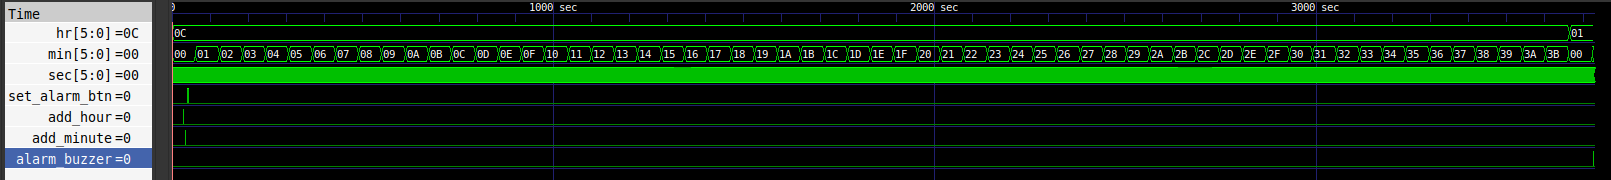
\includegraphics[width=0.7\textwidth]{figs/alarmtest.png}
\end{figure}
\subsection{Timer}
\begin{figure}[H]
    \centering
    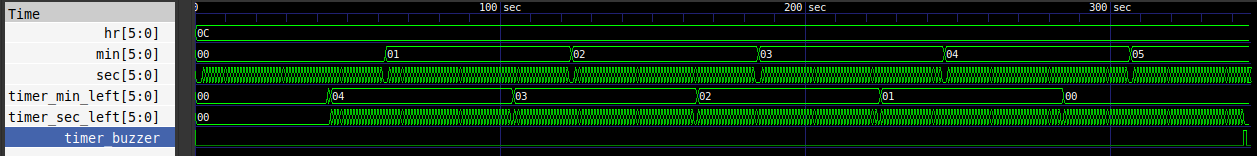
\includegraphics[width=0.7\textwidth]{figs/timertest.png}
\end{figure}
\subsection{Display}
\begin{figure}[H]
    \centering
    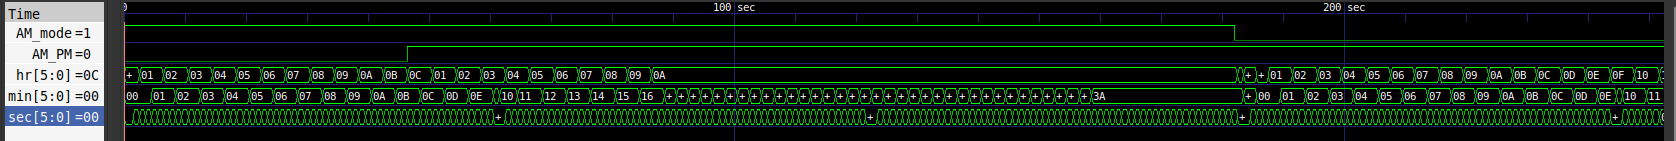
\includegraphics[width=0.7\textwidth]{figs/disptest.png}
\end{figure}
For codes refer to \url{https://github.com/ArnavYadnopavit/FinalProjectDSLab}\\

\centering
Thank You
\end{document}

